\documentclass[]{article}
\usepackage{lmodern}
\usepackage{amssymb,amsmath}
\usepackage{ifxetex,ifluatex}
\usepackage{fixltx2e} % provides \textsubscript
\ifnum 0\ifxetex 1\fi\ifluatex 1\fi=0 % if pdftex
  \usepackage[T1]{fontenc}
  \usepackage[utf8]{inputenc}
\else % if luatex or xelatex
  \ifxetex
    \usepackage{mathspec}
  \else
    \usepackage{fontspec}
  \fi
  \defaultfontfeatures{Ligatures=TeX,Scale=MatchLowercase}
\fi
% use upquote if available, for straight quotes in verbatim environments
\IfFileExists{upquote.sty}{\usepackage{upquote}}{}
% use microtype if available
\IfFileExists{microtype.sty}{%
\usepackage{microtype}
\UseMicrotypeSet[protrusion]{basicmath} % disable protrusion for tt fonts
}{}
\usepackage[margin=1in]{geometry}
\usepackage{hyperref}
\hypersetup{unicode=true,
            pdftitle={PCB sub sampling simulation},
            pdfauthor={Xuelong Wang},
            pdfborder={0 0 0},
            breaklinks=true}
\urlstyle{same}  % don't use monospace font for urls
\usepackage{graphicx,grffile}
\makeatletter
\def\maxwidth{\ifdim\Gin@nat@width>\linewidth\linewidth\else\Gin@nat@width\fi}
\def\maxheight{\ifdim\Gin@nat@height>\textheight\textheight\else\Gin@nat@height\fi}
\makeatother
% Scale images if necessary, so that they will not overflow the page
% margins by default, and it is still possible to overwrite the defaults
% using explicit options in \includegraphics[width, height, ...]{}
\setkeys{Gin}{width=\maxwidth,height=\maxheight,keepaspectratio}
\IfFileExists{parskip.sty}{%
\usepackage{parskip}
}{% else
\setlength{\parindent}{0pt}
\setlength{\parskip}{6pt plus 2pt minus 1pt}
}
\setlength{\emergencystretch}{3em}  % prevent overfull lines
\providecommand{\tightlist}{%
  \setlength{\itemsep}{0pt}\setlength{\parskip}{0pt}}
\setcounter{secnumdepth}{5}
% Redefines (sub)paragraphs to behave more like sections
\ifx\paragraph\undefined\else
\let\oldparagraph\paragraph
\renewcommand{\paragraph}[1]{\oldparagraph{#1}\mbox{}}
\fi
\ifx\subparagraph\undefined\else
\let\oldsubparagraph\subparagraph
\renewcommand{\subparagraph}[1]{\oldsubparagraph{#1}\mbox{}}
\fi

%%% Use protect on footnotes to avoid problems with footnotes in titles
\let\rmarkdownfootnote\footnote%
\def\footnote{\protect\rmarkdownfootnote}

%%% Change title format to be more compact
\usepackage{titling}

% Create subtitle command for use in maketitle
\providecommand{\subtitle}[1]{
  \posttitle{
    \begin{center}\large#1\end{center}
    }
}

\setlength{\droptitle}{-2em}

  \title{PCB sub sampling simulation}
    \pretitle{\vspace{\droptitle}\centering\huge}
  \posttitle{\par}
    \author{Xuelong Wang}
    \preauthor{\centering\large\emph}
  \postauthor{\par}
      \predate{\centering\large\emph}
  \postdate{\par}
    \date{2019-09-03}

\usepackage{float,amsmath, bbm, siunitx, bm}
\usepackage{pdfpages}
\floatplacement{figure}{H}
\newcommand{\indep}{\rotatebox[origin=c]{90}{$\models$}}

\begin{document}
\maketitle

{
\setcounter{tocdepth}{2}
\tableofcontents
}
\section{Motivation}\label{motivation}

Based on the previous simulation results, we found that after using the
historical data to decorrelate the data, the covariates still have some
low correlations among them. But it seems that GCTA and EigenPrism could
work well even the covariate have some low correlations among them. To
further mimic the real data situation, we using the combined PCBs 1999 -
2004 data to simulate the high dimensional data and try to estimate the
combined total vairance by using GCTA and EigenPrism.

\section{Simulation}\label{simulation}

\subsection{Simulation result}\label{simulation-result}

\subsubsection{Chi}\label{chi}

\begin{itemize}
\tightlist
\item
  \(cov(X) = cor(PCB|year = 1999)\)
\item
  \(p = 21\)
\item
  target is the combined main and interaction effect
\item
  X \textasciitilde{} \(\chi^2_1\)
\item
  \(n = 100, 150, 231\)
\end{itemize}

\begin{verbatim}
      n MSE est_var est_mean NA_total     method total decor x_dist
 1: 100  82      66       18        0 EigenPrism    14 FALSE    chi
 2: 150 110      72       21        0 EigenPrism    14 FALSE    chi
 3: 231 114      64       22        0 EigenPrism    14 FALSE    chi
 4: 100  79      66       18        0       GCTA    14 FALSE    chi
 5: 150 108      77       20        0       GCTA    14 FALSE    chi
 6: 231 124      80       21        0       GCTA    14 FALSE    chi
 7: 100  26      26       13        0 EigenPrism    14  TRUE    chi
 8: 150  24      25       14        0 EigenPrism    14  TRUE    chi
 9: 231  15      15       14        0 EigenPrism    14  TRUE    chi
10: 100  28      27       13        0       GCTA    14  TRUE    chi
11: 150  20      20       14        0       GCTA    14  TRUE    chi
12: 231  14      14       14        0       GCTA    14  TRUE    chi
\end{verbatim}

\subsubsection{PCBs}\label{pcbs}

\begin{itemize}
\tightlist
\item
  X: will be 21 PCBs or after adding interaction terms 231
\item
  n: 100,150,231
\item
  traget: \(\beta^T\hat{\Sigma}_h\beta\). Since we don't know the extact
  covariance matrix of the PCBs so we are using the all the historical
  data to estate the covariance matrix \(\hat{\Sigma}_h\)
\end{itemize}

\begin{verbatim}
      n MSE est_var est_mean NA_total     method total decor x_dist
 1: 100 193     134     19.0        4 EigenPrism    11 FALSE   1999
 2: 150 483     332     23.7        0 EigenPrism    11 FALSE   1999
 3: 231 320     177     23.3        0 EigenPrism    11 FALSE   1999
 4: 100 153     132     15.9        0       GCTA    11 FALSE   1999
 5: 150 693     587     21.8        0       GCTA    11 FALSE   1999
 6: 231 292     194     21.2        0       GCTA    11 FALSE   1999
 7: 100  47      47     10.9        0 EigenPrism    11  TRUE   1999
 8: 150  37      37     10.7        0 EigenPrism    11  TRUE   1999
 9: 231  18      15      9.5        0 EigenPrism    11  TRUE   1999
10: 100  50      49     10.1        0       GCTA    11  TRUE   1999
11: 150  39      39     10.2        0       GCTA    11  TRUE   1999
12: 231  18      16      9.5        0       GCTA    11  TRUE   1999
\end{verbatim}

\newpage

\paragraph{Simulation result with larger
n}\label{simulation-result-with-larger-n}

If we subset data as the corresponding years, then it seems that we can
get covariance matrix which is very close to \(I\). However, if the size
of the sub-sample is small, e.i.100, then the decorrelated covariance
matrix may be not close to \(I\)

\begin{itemize}
\tightlist
\item
  \(n \in \{100, 500, 1000, 2000\}\)
\end{itemize}

\begin{figure}
\centering
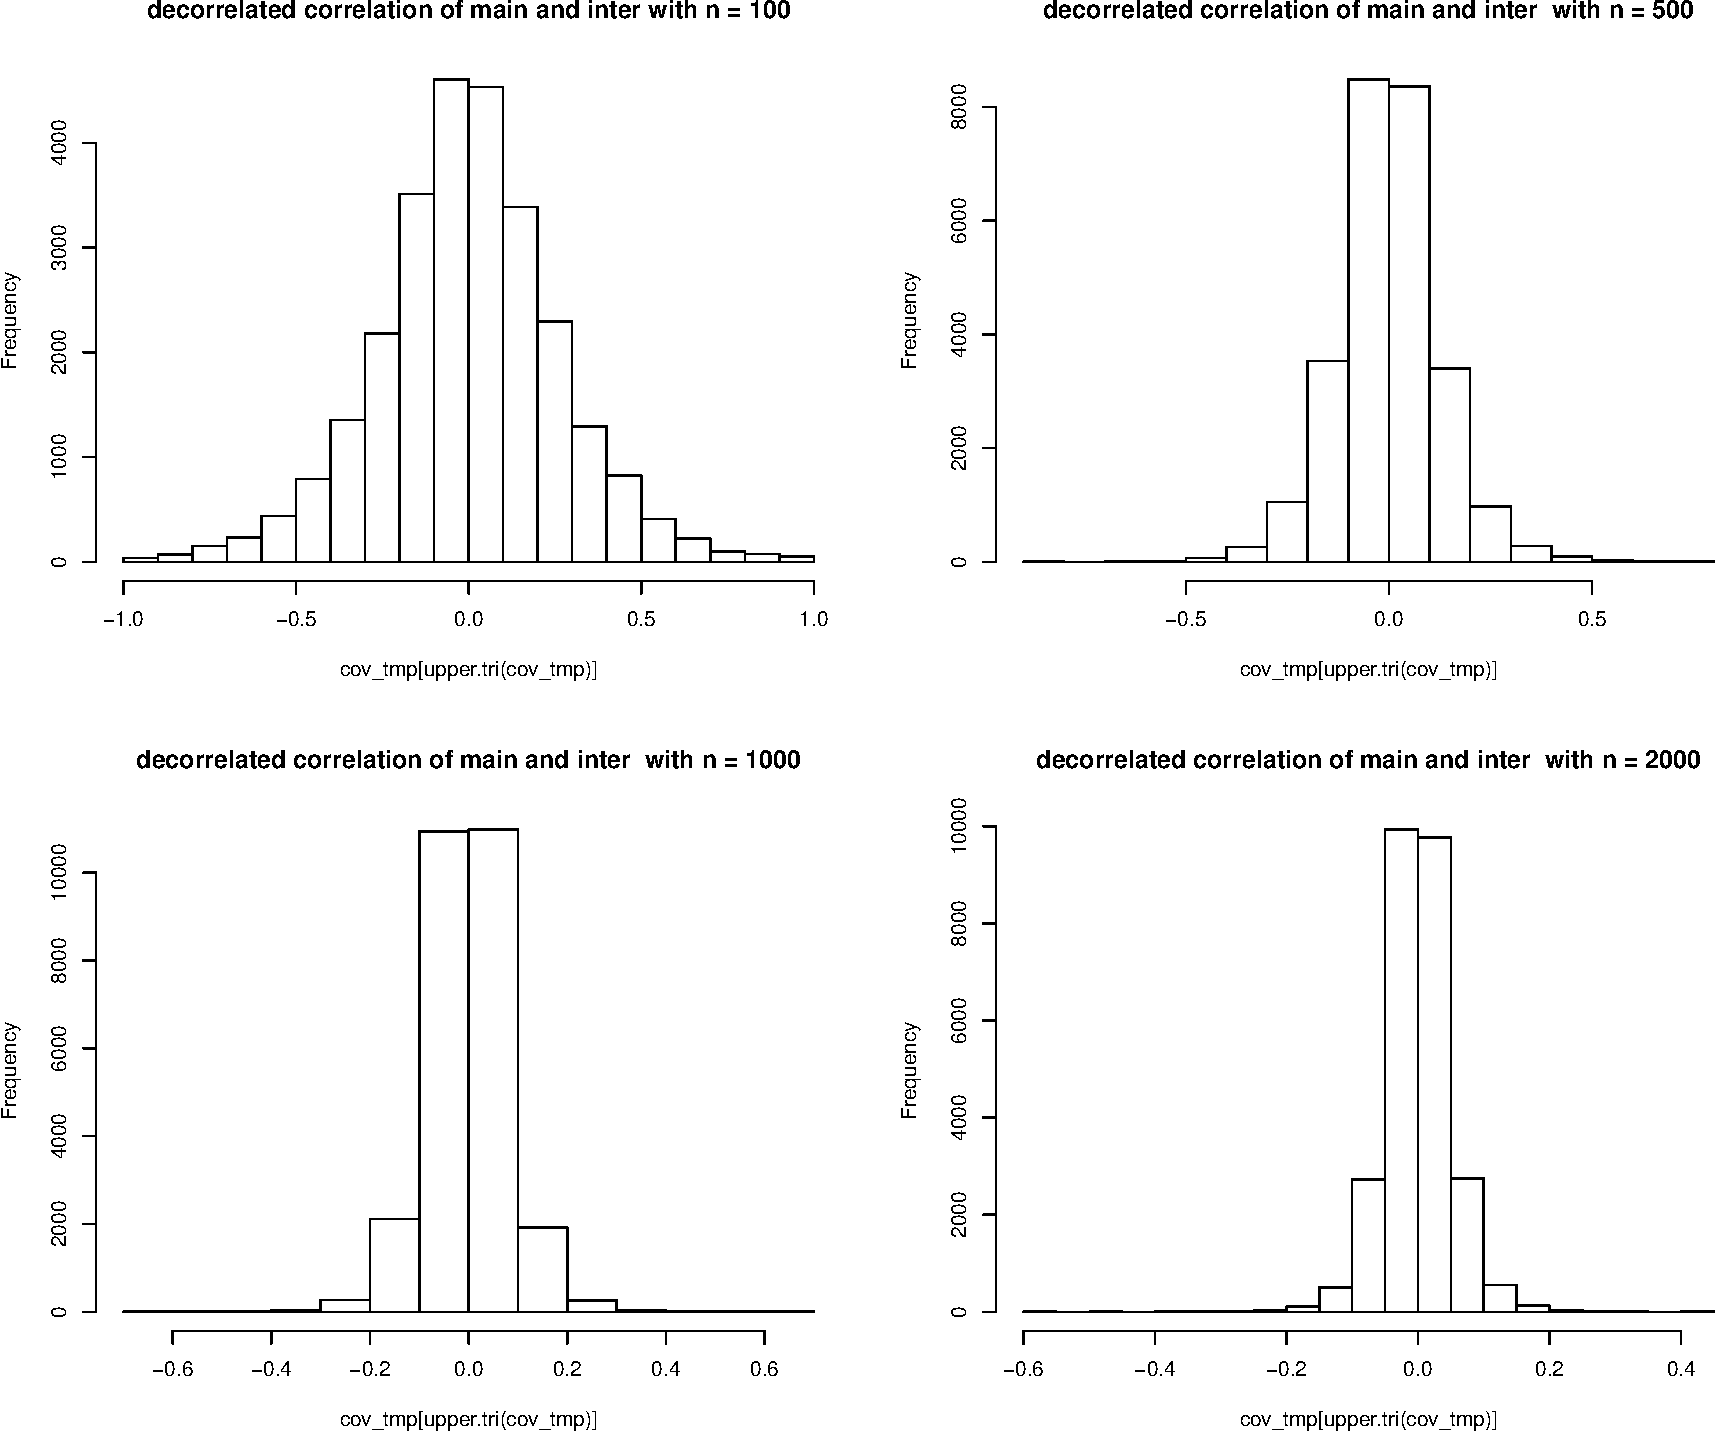
\includegraphics{PCBs_covariance_subsampling_files/figure-latex/unnamed-chunk-3-1.pdf}
\caption{Combined main and interaction 1999-2000}
\end{figure}

\begin{verbatim}
      n  MSE est_var est_mean NA_total method total decor x_dist
1:  100 49.9    49.1     10.1        0   GCTA    11  TRUE   1999
2:  500 11.2     9.2      9.8        0   GCTA    11  TRUE   1999
3: 1000  6.9     5.0      9.9        1   GCTA    11  TRUE   1999
4: 2000  3.8     2.4     10.0        2   GCTA    11  TRUE   1999
\end{verbatim}

\section{problems}\label{problems}

\subsection{Interaction and
decorrelation}\label{interaction-and-decorrelation}

The procedure to generate and estimate the combined main and interaction
effect is followings:

\begin{enumerate}
\def\labelenumi{\arabic{enumi}.}
\tightlist
\item
  \(X \rightarrow X_t = (X, X_{inter}) \rightarrow Y = X^t\beta_t + \epsilon\)
\item
  \(X \rightarrow X_t = (X, X_{inter}) \rightarrow Z_t = X_t^T \Sigma_h^{-1/2} \rightarrow \hat{Var}(X_t^T\beta_t)\)
\end{enumerate}

The problem I encounter is that if I did not standerdize the PCBs then
it seems that the estimated combined effect is close to the target even
if we don't apply the decorrelation procedure.

\begin{verbatim}
      n MSE est_var est_mean NA_total     method total decor x_dist
 1: 100 129     112     10.5        1 EigenPrism    15 FALSE   1999
 2: 150 221     219     12.8        0 EigenPrism    15 FALSE   1999
 3: 231 126     114     11.2        0 EigenPrism    15 FALSE   1999
 4: 100  88      55      9.1        0       GCTA    15 FALSE   1999
 5: 150 207     190     10.4        0       GCTA    15 FALSE   1999
 6: 231  93      63      9.3        0       GCTA    15 FALSE   1999
 7: 100  97      82     10.8        0 EigenPrism    15  TRUE   1999
 8: 150 114      99     10.8        0 EigenPrism    15  TRUE   1999
 9: 231  61      28      9.1        0 EigenPrism    15  TRUE   1999
10: 100 132     113     10.3        0       GCTA    15  TRUE   1999
11: 150 130     113     10.6        0       GCTA    15  TRUE   1999
12: 231  64      31      9.1        0       GCTA    15  TRUE   1999
\end{verbatim}

After some simulation, I found it is possible because of the small
values of the PCBs. Although the correlation of PBCs are high, the
covariance of PCBs are small because of the small values of PCB.
decorerlation i


\end{document}
